%! TEX root = ../main.tex
% ==============================================================
% IMMUTABLE — generated automatically, do not edit this block
%
% — Provenance ───────────────────────────────────────────────────
%   script            : analysis_scratch/inspirational_timeseries.py
%   computed_in       : analysis_scratch/inspirational_timeseries.py (single-run time-series render)
%   plot_type         : inspirational_timeseries
%   data_class        : DELEG
%   generated_at      : 2026-04-24T12:20:10
%   findings_doc      : memory/methodology_hg_window_kills_peak_bias.md
%
% — Thesis context ──────────────────────────────────────────────
%   chapter           : 04
%   caption_label     : fig:ch04_inspirational_fullwind
%   caption_short     : 
%
% — Filters ────────────────────────────────────────────────────
%   panel             : full
%   wind              : full
%   amplitude [V]     : 0.2
%   frequency [Hz]    : 1.4
%   probes            : 
%   run_category      : 
%   quality_flag      : ok
%   mooring           : 
%
% — Data provenance ────────────────────────────────────────────
%   n_runs            : 
%   in_probes_used    : 
%   out_probes_used   : 
%   probe_configs     : 
%   non_final_config_n: 
%   datasets        :
%     PROCESSED-20251005-sixttry6roof-highMooring
%     PROCESSED-20251110-tett6roof-lowM-ekte580
%     PROCESSED-20251110-tett6roof-lowMooring
%     PROCESSED-20251110-tett6roof-lowMooring-2
%     PROCESSED-20251112-tett6roof
%     PROCESSED-20251113-tett6roof
%     PROCESSED-20251113-tett6roof-loosepaneltaped
%     PROCESSED-20251113-tett6roof-probeadjusted
%     PROCESSED-20260305-newProbePos-tett6roof
%     PROCESSED-20260306-newProbePos-tett6roof
%     PROCESSED-20260307-ProbPos4_31_FPV_2-tett6roof
%     PROCESSED-20260312-ProbPos4_31_FPV_2-tett6roof
%     PROCESSED-20260313-ProbePos4_31_FPV_2-tett6roof
%     PROCESSED-20260314-ProbePos4_31_FPV_2-tett6roof
%     PROCESSED-20260316-ProbePos4_31_FPV_2-tett6roof
%     PROCESSED-20260316-ProbePos4_31_FPV_2-tett6roof-under9Mooring
%     PROCESSED-20260319-ProbePos4_31_FPV_2-tett6roof-under9Mooring
%     PROCESSED-20260321-ProbePos4_31_FPV_2-tett6roof-under9Mooring-height100-RENAMED
%     PROCESSED-20260323-ProbePos4_31_FPV_2-tett6roof-under9Mooring-height100
%     PROCESSED-20260323-ProbePos4_31_FPV_2-tett6roof-under9Mooring-height136
%     PROCESSED-20260324-ProbePos4_31_FPV_2-tett6roof-under9Mooring-height100
%     PROCESSED-20260325-ProbePos4_31_FPV_2-tett6roof-under9Mooring-height100
%     PROCESSED-20260326-ProbePos4_31_FPV_2-tett6roof-under9Mooring-height100
%     PROCESSED-20260326-ProbePos4_31_FPV_2-tett6roof-under9Mooring-height100-lowrange
%     PROCESSED-20260327-ProbePos4_31_FPV_2-tett6roof-under9Mooring30-height100-lowrange
%   run_paths       :
%     (omitted — aggregate over > threshold runs, see datasets)
%
% — Method / numerical parameters ─────────────────────────────
%   grouper           : 
%   collapse_panels   : 
%   fft_window_hz     : 0.1
%   extra_params      : run_path=wavedata/20260327-ProbePos4_31_FPV_2-tett6roof-under9Mooring30-height100-lowrange/fullpanel-fullwind-amp0200-freq1400-per240-depth580-mstop30-run1.csv. probes=IN:9373/170+OUT:12400/250. zoom=5 periods centred on each probe's H&G window (macro = full recording, ~52.6 s cutoff). H&G window: probe-shifted [50T, 60T] anchored at r = 12.4 m, IN shifted earlier by group-velocity Δt; start UC-snapped within ±T, end UC-snapped to the 10th upcrossing with ±0.5 T guard. Amber vspan on macro = zoom extent; zoom extent is a 5-period window centred on each probe's own H&G window midpoint so OUT zoom sits later in time (wave-group lag). Colour convention: blue = nowind, red = fullwind — CLAUDE.md thesis-wide WIND_COLOR_MAP. Typeset in NewComputerModern10 (OTFs from TeXLive's newcomputermodern package, registered via font_manager).
%
% — Summary stats cited in caption ────────────────────────────
%   stat:ka_inn       : 0.1511
%   stat:ka_Ut        : 0.0994
%   stat:A_inn_FFT_mm : 15.742
%   stat:wavelength_inn_m : 0.7969
%   stat:wavenumber_inn_per_m : 7.8852
%   stat:period_inn_s : 0.71460
%   stat:celerity_inn_m_s : 1.1151
%   stat:Hm0_inn_mm   : 46.142
%   stat:Hs_inn_mm    : 37.388
%   stat:Froude_inn   : 0.21999
%   stat:Ursell_inn   : 0.12480
%   stat:wind_over_c_inn : 5.2014
%   stat:f_over_fPM_inn : 5.3355
%   stat:wave_stability_inn : 0.8723
%   stat:period_cv_inn : 0.0654
%   stat:A_Ut_FFT_mm  : 11.729
%   stat:wavelength_Ut_m : 0.7937
%   stat:wavenumber_Ut_per_m : 7.9160
%   stat:period_Ut_s  : 0.71320
%   stat:celerity_Ut_m_s : 1.1129
%   stat:Hm0_Ut_mm    : 33.384
%   stat:Hs_Ut_mm     : 25.200
%   stat:Froude_Ut    : 0.21956
%   stat:Ursell_Ut    : 0.08111
%   stat:wind_over_c_Ut : 5.2115
%   stat:f_over_fPM_Ut : 5.3459
%   stat:wave_stability_Ut : 0.8889
%   stat:period_cv_Ut : 0.0421
%   stat:A_inn_LS_mm  : 16.055
%   stat:A_inn_Stk2_mm : 1.418
%   stat:A_inn_percentile_mm : 18.531
%   stat:A_inn_PSD_mm : 15.990
%   stat:A_inn_cycles_mean : 16.878
%   stat:A_inn_phase_mean : 14.872
%   stat:DC_inn_mm    : 0.6828
%   stat:residualRMS_inn_mm : 2.2619
%   stat:window_inn_s : [30.552, 37.676]
%   stat:hg_snap_shift_inn_samples : 46.0
%   stat:A_Ut_LS_mm   : 11.719
%   stat:A_Ut_Stk2_mm : 0.861
%   stat:A_Ut_percentile_mm : 12.560
%   stat:A_Ut_PSD_mm  : 11.682
%   stat:A_Ut_cycles_mean : 12.108
%   stat:A_Ut_phase_mean : 11.739
%   stat:DC_Ut_mm     : 0.3281
%   stat:residualRMS_Ut_mm : 0.6922
%   stat:window_Ut_s  : [35.444, 42.572]
%   stat:hg_snap_shift_Ut_samples : -89.0
%   stat:meta_OUT_over_IN : 0.7451
%   stat:file_date    : 2026-03-27
%   stat:mooring      : below_90_loose300
%   stat:probe_height_mm : 100.0
%   stat:probe_range_mode : low
%   stat:water_depth_mm : 580.0
%   stat:kd_Ut        : 4.591
%   stat:depth_regime : deep
%   stat:input_freq_Hz : 1.40
%   stat:input_amp_V  : 0.20
%   stat:sampling_rate_Hz : 250.0
%   stat:zoom_periods : 5
%   stat:wind_condition : fullwind
%
% — Subfigures available ───────────────────────────────────────
%     FIGURES/ch04_inspirational_fullwind.pdf
% ── end immutable block ─────────────────────────────────────────
\begin{figure}[htbp]
  \centering
  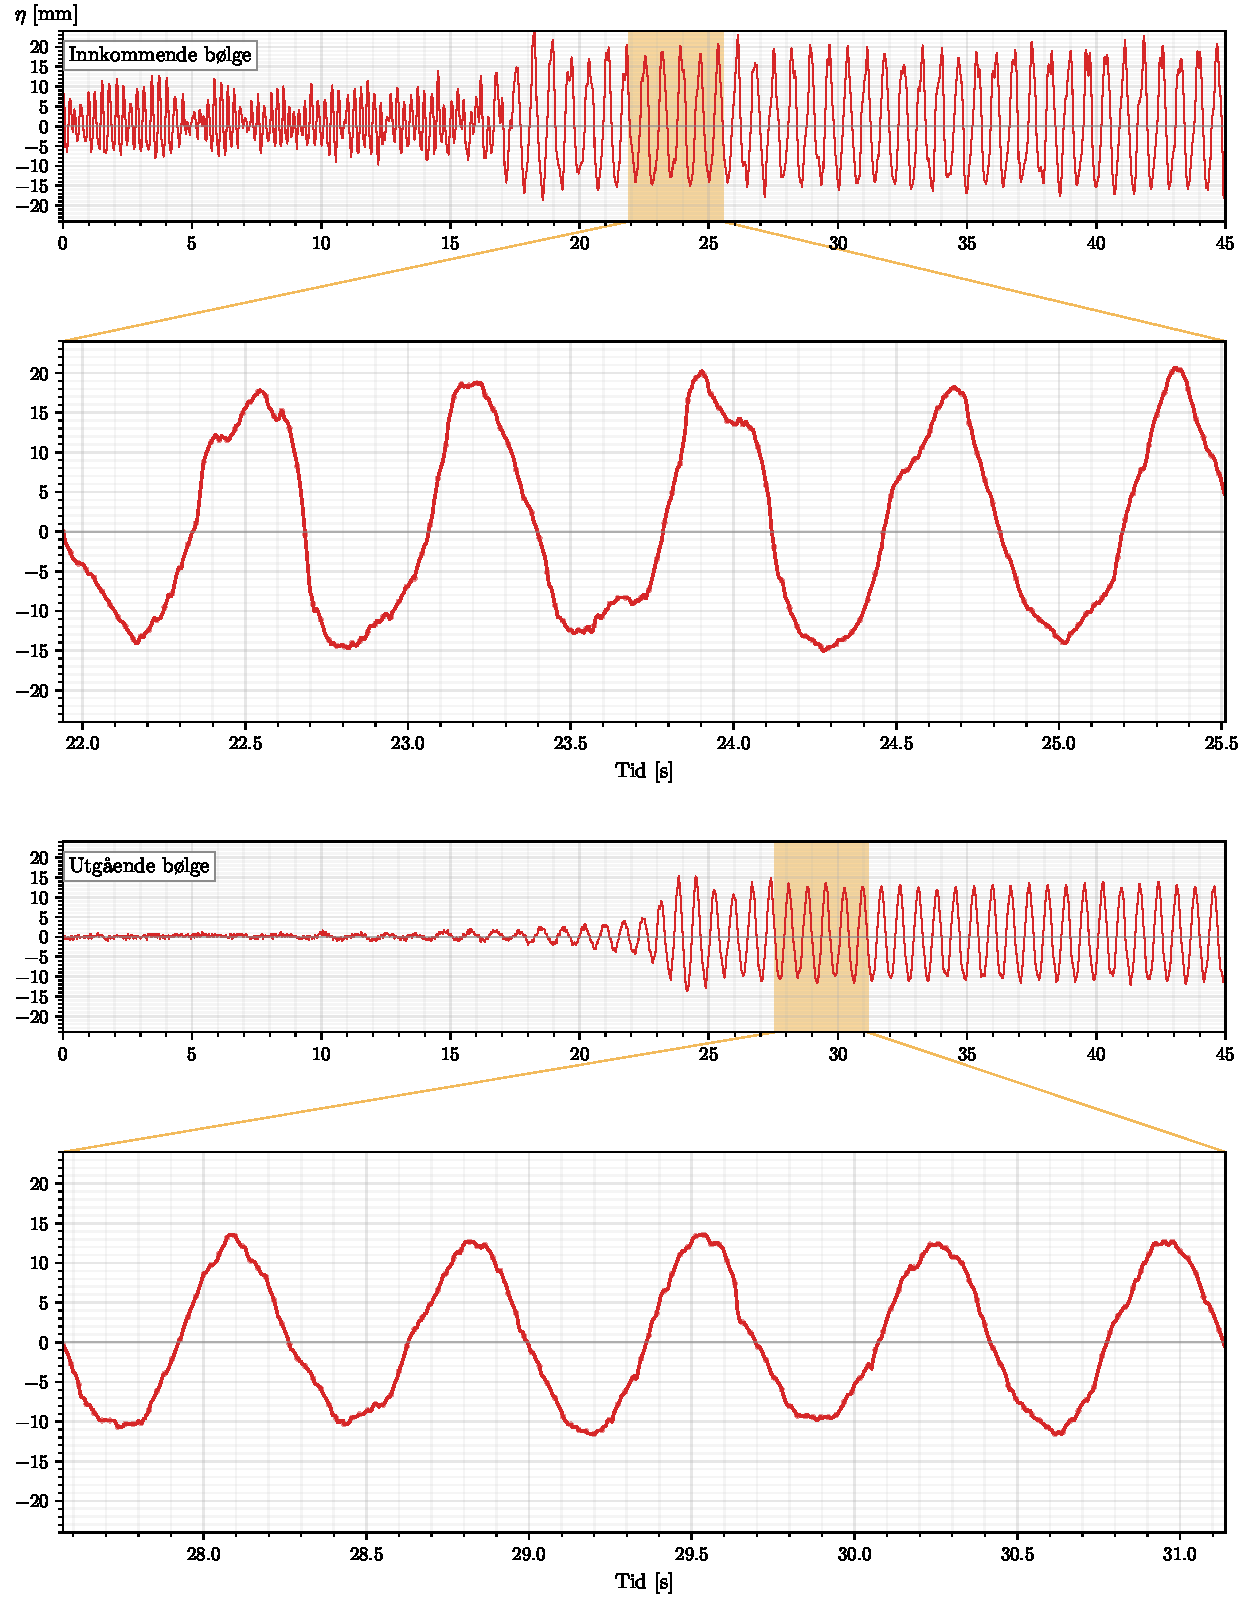
\includegraphics[width=0.9\linewidth]{FIGURES/ch04_inspirational_fullwind.pdf}
  \caption[Short caption for LOF]{
    % TODO: write caption
  }
  \label{fig:ch04_inspirational_fullwind}
\end{figure}
